\chapter{General Semistructured Model and Nested Graphs}\label{cha:graphsdef}
\epigraph{``\textit{The empirical basis of objective science has nothing 'absolute' about it. Science does not rest upon solid bedrock. The bold structure of its theories rises, as it were, above a swamp. It is like a building erected on piles. The piles are driven down from above into the swamp, but not down to any natural or 'given' base; and if we stop driving the piles deeper, it is not because we have reached firm ground. We simply stop when we are satisfied that the piles are firm enough to carry the structure, at least for the time being.}''}{--- Karl R. Popper, \textit{The Logic of Scientific Discovery}, V. 30}

%The previous chapter showed that better performances for graph algorithms can be performed by using an adjacency list representation. This implementation provided better performances that the ones achievable on both relational and graph data storages, and that our proposed query plan performed better solutions that the one provided by current graph query languages. Nevertheless, in 

Chapter \vref{cha:datadef}  addressed the problem of providing nested concepts in current data models. Graph models also proved not to meet such representation goals adequately and, therefore, a new data model for graph nested data is required. On the other hand, semistructured data representations do not allow to represent the containment of one single object by multiple containers, as needed for a possible generalization of the EPGM\index{graph!EPGM} model. Consequently, we choose to first define of a generalized semistructured data representation (\textbf{GSM}\index{GSM|see {General Semistructured Model}}\index{General Semistructured Model}, Section \ref{def:mofgeneral}) on top of which the new nested graph model is going to be subsequently defined (\textbf{nested graphs}\index{graph!nested graphs}, Section \ref{def:ngraph}). 

The present chapter provides some translation functions $\tau$ from the previous data models towards the GSM data model, thus meeting twos distinct goals: \begin{mylist}
	\item we show the generality of GSM, that
	\item can be the used within the LAV/GAV \index{data integration!global as a view} \index{data integration!local as a view} data integration scenarios for syntactically translating one data model towards the GSM or Nested Graph model, thus defining $\ttransl$.
\end{mylist}
The choice of representing both vertices and edges with ``objects''\index{object} may surprise the reader, because Chapter \ref{cha:datadef} warned against the problem of semantic overloading. The reader must be aware that the implications of the previous paragraph fall only at the representation level of the single element while, on the other hand, the data model should distinguish between all those different concepts.


\begin{figure}
	\centering
	\begin{minipage}{.45\textwidth}
		\centering
		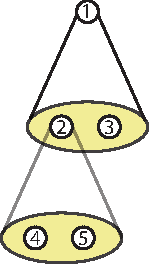
\includegraphics{fig/04model/01SimpleNesting}
		\subcaption{This picture provides a representation of a data structure containing two different nesting levels. Each object is represented by a circle, while
			the containment $\varphi$ function of each object is represented by the cone departing from each object. Within this graphical representation, the leftmost nested object is the first object appearing in the containment function $\varphi$.}
		\label{fig:01simplenesting}
	\end{minipage}\quad \begin{minipage}{.45\textwidth}
		\centering
		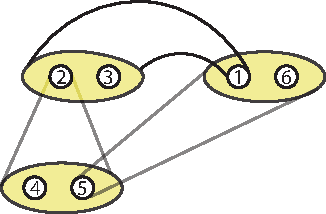
\includegraphics{fig/04model/02RecursiveNesting}
		\subcaption{The data model that is now provided is as general as possible, and hence can support any possible representation. This also implies that recursive nestings are allowed. In particular, this Figure shows that node $2$ may contain elements $4$ and $5$, which contains $6$ and $1$ which contains $1$ back. Therefore, $\varphi(2)=[4,5]$, $\varphi^2(2)=[1,6]=\varphi(5)$, and $\varphi^3(2)=[2,3]$. This recursive nesting solutions should be avoided for representing aggregations.}
		\label{fig:02recursivenesting}
	\end{minipage}%
	\bigskip 
	
	\begin{minipage}{.45\textwidth}
		\centering
		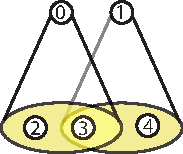
\includegraphics{fig/04model/03Overlapping}
		\subcaption{This picture shows how the $GSM$ model allows to nest one element (e.g. $3$) in more than one single element. In particular, $\phi(0)\cap\phi(1)=[3]$.}
		\label{fig:03overlapping}
	\end{minipage}
	\caption{Different possible instances of the $GSM$ model, allowing arbitrary nestings within its objects. These pictures show some situations that cannot be natively expressed by the current nested relational model and other semistructured representations. In particular, each cone represents one single association between the containing object and its content through an expression $p$.}
\end{figure}
Last, we provide some use cases for both aggregating (Section \ref{subsec:nested-partof}) and integrating (Section \ref{sec:ngusecases}) data representations within the proposed data format. Concerning the last use case, we must previously observe that in the third chapter  we  showed that the alignment of types -- which may nest other concepts -- relies on both the successive alignment of other attributes (or nested types) and on the attributes contained inside such types. Given that both types and attributes are involved in the alignment process, it follows that they all must be represented -- within the alignment process -- as objects with a given type represented through labels. 
After this alignment process, edges must be aligned too: this process is required for a complete data integration scenario. Consequently, this chapter introduces the concept of edge alignment for data integration (as previously introduced in Section \vref{sss:ngdi}), thus allowing to provide a first definition of the $\qtransl$ operator as well as $\ttransl$ over the previously mined alignments. Moreover, the same example shows that GSM allows a uniform representation between data models, schemas and alignments.

%\texttt{Although most of the strengths of the relational data model rely upon a well-established 
%theory \cite{Codd} and many textbooks have been published on this subject \cite{Garcia-Molina}, this 
%doesn't necessarily mean that relational data management systems have to be the only possible solution to
%store data. This assertion is more evident while looking at the problems of the overmentioned model
%(Section \ref{sec:relproblems}). Consequently, two different solutions were adopted: the first one was to
%provide a further relaxation to the data model by providing semi-structured data, and the second one
%was the definition of the Object-Oriented DBMSs. In particular semi-structured data could be represented 
%with NoSQL data models, where graph databases are also included as a specific case (Section \ref{sec:NoSQL}). 
%We are also going to show that such NoSQL models provide partial solutions to the relational model issues.
%
%It should be clear that none
%of NoSQL solutions has to be considered generally ``better'' than the relational data model, 
%since the proposed solutions try to provide a more appropriate data representation approach
%for specific problems and issues.
%
%
%\section{Problems of the Relational Data model}
%\label{sec:relproblems}
%In this section we show both the well-known problems of the relational data model, and 
%how such problems were solved in NoSQL data models. Moreover, we are going to show how 
%such models could be ever represented through a graph data model. 
%
%\phparagraph{Data Representation Problems}
%One of the most evident problems of relational data models relies on their inability of providing
%an efficient representation of \textit{semi-structured data}: for this reason XML has been used to overcome to this
%problem. Some languages have been proposed to query such data representation: \textbf{XPath} \cite{xpath31} and \textbf{XQuery} \cite{XQuery} are 
%the most used languages in this field: the first one implements traversal queries
%that are used in the second language, which is functional and expression-oriented. Other different solutions
%\cite{magnani04,Lu,magnani06} have been proposed to query such data structure through algebraic operators,
%with the aim of integrating semistructured with structured data. None of these solutions has been implemented yet. On the other hand
%there are no data integration systems for graph data, but many different graph query languages have been implemented 
%(see Section \vref{sec:dbqlang}), that could carry out either data manipulation or perform path traversal, or both solutions
%at the same time. Even if usually hypertext contents are represented through semi-structured data such as XMLs \cite{IorioHierarchy}, some recent work have proposed to express such contents in a graph form \cite{BarabucciEARMARK},
%over which is possible to run automatic reasoners like \textbf{Jena} \cite{Jena} and \textbf{Pellet} \cite{Pellet}, that
%subsume a specific graph data model, RDF \cite{Lassila1999,GutierrezInclusion}.
%
%The main difference between XML and tree data and Graph Data is that the second one provides a more reliable representation of the 
%data topology \cite{Gut08}, since it allows any possible connection between the nodes. Even if both edges and nodes
%could be labelled and hence store information, graph data representation assumes that all the relation between the vertices 
%are binary.
%The need of more general relations s confirmed by the fact that complex systems often show n-ary relations \cite{Johnson2011} and that
%specific Artificial Intelligence applications used hypergraph databases to both keep track of the reasoning processes
%and to express the ``queries'' over this data representation \cite{OpenCog1}. Despite most of the hypergraph problems
%could be reduced to graph problems and that literature has already provided some results in this regard \cite{ausiello},
%this data model currently does not have a vast and large diffusion as tree (XML) and graph representation of data.
%
%Even if XML was originally designed to represent tree data structures, it could be easily represent graph data representations via
%specific Document Type Definitions, because XML is a meta-markup language. \textbf{GraphML} \cite{graphml} and \textbf{GXL} \cite{gxlgraphml} are examples of possible ways to express graphs through inside a semi-structured data format.
%
%\phparagraph{Object Identity}
%In the relational data model, even if the user-defined primary key could be associated to a specific row,
%two different keys could be used could be used to identify two different relational table's rows presenting the
%same values when no specific constraint are specified. This phenomenon does not arise in the RDF data model,
%since each node is associated to an unique URI identifier \cite{GutierrezInclusion}, while this currently
%happens in graph databases that are based on the \textit{property graph} model, where each node is generally
%described as a tuple \cite{Neo4jAlg}. Consequently, the vertex indexing function is not used as an unique object identifier and 
%it is used to provide quick access to the data resources.  
%
% besides the user-defined primary key that could be associated to a specific row, 
%there is no independent identification of each row when conceived as an entity. As a result, modern RDBMSs allow
%data replication and hence conflicts could arise while updating multiple instances of the same given entity. This 
%problem persists in the property graph model since no specific constraint are given to characterize a node as a
%specific entity, and consequently multiple instances of the same node could coexist. The same phenomenon happens
%for data represented in XML format, while RDF graphs are designed to represent each node and each labelled edge between two
%nodes only once. 
%
%The Object Identity problem has already been formulated and solved by the Object-Oriented data model: for each object
%representing an instance of a relation $\Re$, the unique identifier could be uniquely determined via a function $f_\Re$ 
%(called \textit{Skolem Functor}) which computes the unique id from the object's terms \cite{Cabibbo}. With this function
%it is possible to generate new IDs for each newly created objects. Consequently, such objects could be easily implemented
%in current programming languages (e.g. Java) where both hashing functions and equivalence predicates are provided for
%each class. 
%
%\phparagraph{Explicit Relationships}
%Even if the ER model \cite{Chen1976} provides a graph-oriented description of the data where both entities and relations
%are explicitly stated, its translation into the relational model flattens both entities and relations into a uniform tabular
%representation. In order to recover such relationships, we have to explicitly perform queries over the relational
%database. 
%The same problem persists in the semi-structured data model:
%even if in the XML data model there is a notion of hierarchy through the nesting of the tag elements, there is
%no uniform and explicit semantics to describe which is a possible interpretation of the elements' nesting. 
%
%In order to
%explicitly state the kind of relation that undergoes between such tags, a graph representation of such data is required
%\cite{IorioHierarchy}. Moreover, graph databases could be used to express hierarchies and other relations among the data
%through ontologies \cite{EtcheverryV12b}, and hence could be used to provide a multidimensional representation of the
%data. 
%
%\phparagraph{Recursive queries}
%An early extension of the relational algebra \cite{AhoAlpha} tried to extend such algebra with an operator,
%that provided a transitive closure over the directed binary relations stored in relational tables through a fixpoint 
%evaluation. As we could see from the
%previous discussions, the implementation of object identifiers is prerequisite for checking whether the vertices have
%been already visited or not: such idea was adopted during the definition in order to check whether new records were
%visited or not. This fix-point operator would be later named $\alpha$ \cite{Alpha}. 
%
%Recursive queries became standard with 
% \textbf{SQL:1999}, where a \texttt{WITH RECURSIVE} was added to the SQL syntax, A least fix-point
% semantic was associated to this clause. 
% The implementation of the $\beta$ operator for graphs \cite{gomesjrhal}, direct descendant of the 
%$\alpha$ operator, is an exact application of this regard.
%
%\phparagraph{Generalization and Inheritance}
%Similarly to what was stated previously for explicit relationships, ER model expresses inheritance relations between the from the former code
%entities that has to be reified in the final relational implementation. While the XML tree data model could express taxonomies,
%graph data structures are more prone to provide a knowledge representation of the data (RDF, \cite{Lassila1999}). Since graph
%data is more prone di describe generalization relations between the data, current automated reasoners work with
%a graph data representation.
%
%
%\section{NoSQL data management systems}\label{sec:NoSQL}
%%[\dots] graph database management systems (GDBMSs from now on) will not be competitive 
%%in a future in terms of theoretic studies, efficiency and technological advancement. 
%Many NoSQL approaches have been proposed: such solutions contrast with the stronly-typed relational database approach.
%\begin{description}
%	\item[KeyValue Database] While relational databases rely upon the storage of rows representing instances
%	of a specific relation, \textit{key-value databases} are a storage paradigm for associative arrays, commonly
%	know as \textit{dictionaries}. Each object is uniquely identified by a key, and hence such key is used
%	to retrieved a specific object. This implementation allows storing data closely following modern object-oriented
%	programming paradigms. \textbf{MonetDB} \cite{MonetDB} is an example of 
%	such kind of NoSQL databases.
%	\item[Document-Oriented Database] \textit{Document-oriented databases} are a specific case of KeyValue databases,
%	where each value is usually a semi-structured document (e.g.\; either XML or JSON). \textbf{CouchDB} is an example of 
%	such kind of NoSQL databases.
%	\item[Column Database] While relational databases rely upon the row representation of the information,
%	the \textit{column databases} ``garner'' the values in a columnar format: the information is serialized
%	by attribute omitting \texttt{NULL}s, and then stored into a column. Consequently, spare information could be
%	stored more efficiently, since each column value is associated to a given row identifier. The most representative system of this kind is \textbf{MonetDB} \cite{MonetDB}. 
%\end{description}
%
%
%%% Che cosa risolve il modello a grafo di questi svantaggi
%In particular, \textit{graph databases} are a specific type of NoSQL databases, since they neither represent
%relational data, nor necessairly use SQL as a querying language (See \cite{SQLGraph} for a counterexample).
%Graph databases could be seen as Document-Oriented databases, where each vertex is a document and a new relation
%layer is added  upon it: consequently, they permit expressing explicit relations unlike the relational model. 
%At this stage we only described the ``pros'' of graph database data model: in the next chapter we are going to
%focus on the current graph query languages and to show their shortcomings.
%
%
%%Nowadays many GDBMSs have been proposed, like \textbf{Neo4J} \cite{Robinson} or \textbf{Titan}.
%%\textbf{Jena} \cite{Jena} and \t{sec:ngusecases}extbf{Pellet} \cite{Pellet} subsume a graph data model over which express both data 
%%and properties.
%
%%%%%%%%%%%%%%%%%%%%%%%%%%%%%%%%%
%}%\part{Testing Part}

%Before introducing a new data structure, we must ask ourselves which is a convenient representation for both providing alignments on nested data structures and  allow data integrations. I Consequently, the user shall be allowed to establish relationships between relations as in the RDF model.

%Given those considerations, it may seem that vertices, edges and attributes should be all represented as objects. 


%%% So, before starting with the description of the new nested graphs (Section \vref{def:ngraph}), we will extend the MetaObject Facility presented in the introductory third chapter, thus providing a general framework for semistructured models (Section \vref{def:mofgeneral}). We will then show how such data model allows to preform the alignment between semistructured data and graphs, representing a hub ontology (Example \vref{ex:examplegraphdata}), thus providing the outline for an algorithm for the integration of any kind of data over nested graphs. After providing some more use cases showing the practical usages (Section \vref{sec:ngusecases}), we will move towards the conclusions, not before that the transformation functions from the other presented data models to the nested graphs are showed (Section \vref{sec:tautonesting}). 
%Such conclusions will introduce the reader to the paNGRAm algebra over nested graphs, that will be introduced in Section \vref{sec:pangramAlgebra}.